Sans entrer dans les détails du code disponible dans les sources je précise quelques spécificités de la transformation.
Le template principal fait appel à d'autres templates pour rendre la lecture du .mtl plus facile et plus modulaire.
Le template différencie bien les read-arc mais il n'est pas possible de préciser un marquage maximal autorisé.\\

Voilà ce que ça donne avec nos deux fichiers pdl convertis en petrinet :

\begin{figure}[h]
\centering
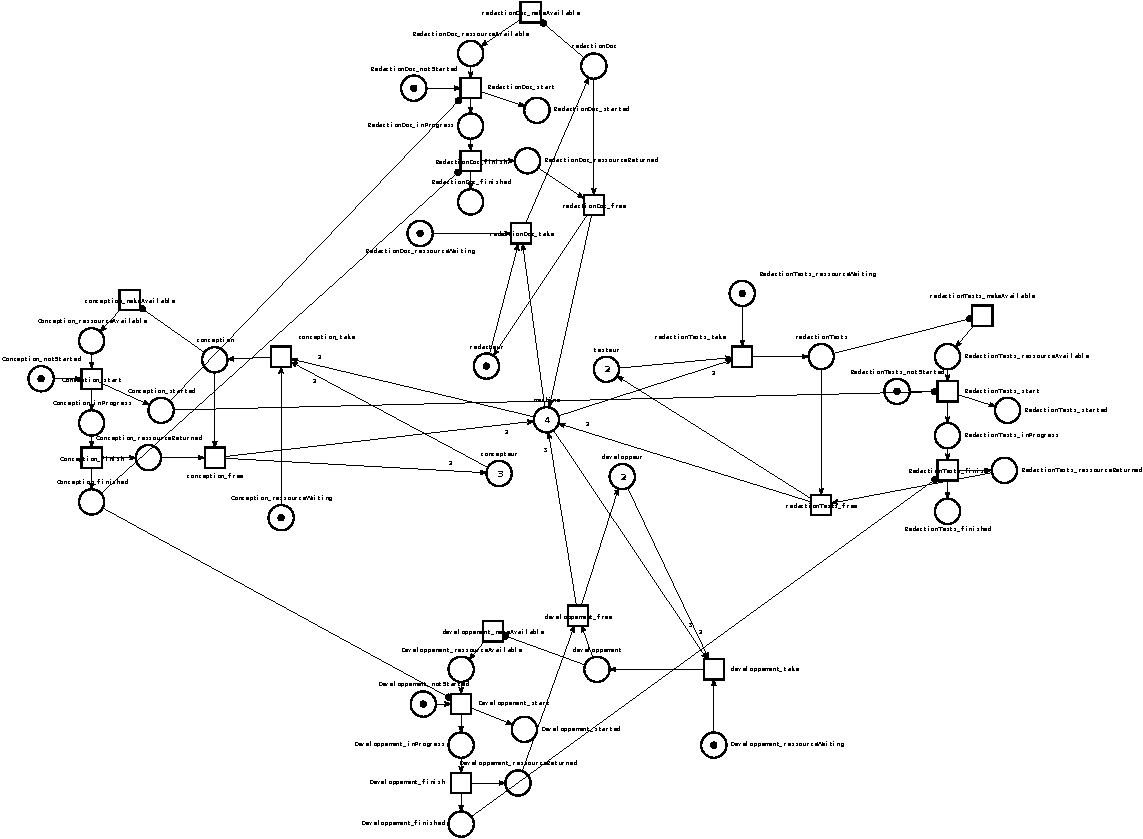
\includegraphics[width=1\textwidth]{../Images/processus_net.pdf}
\caption{Processus tranformé en pétrinet}
\end{figure}

\begin{figure}[h]
\centering
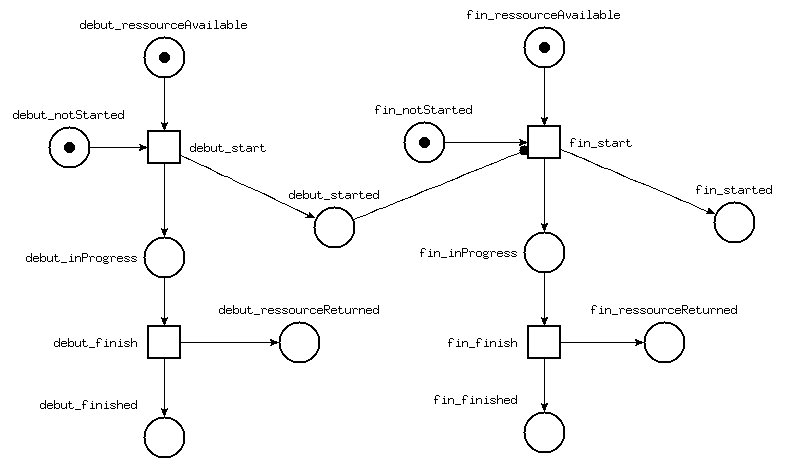
\includegraphics[width=0.45\textwidth]{../Images/model_process_simple_net.png}
\caption{Processus simple tranformé en pétrinet}
\end{figure}
